--- /home/jesse/Analysis/FemtoAnalysis/LamKPublication/CERN/2_EB/EB2/LamKPublication_v5.tex
+++ /home/jesse/Analysis/FemtoAnalysis/LamKPublication/CERN/2_EB/EB2/LamKPublication_v6.tex
@@ -224,17 +224,17 @@
 Additional methods are included to reduce the contamination in the \Kpm samples from the electrons and pions.  
 The specifics for the \Kpm selection are contained in Table~\ref{tab:KchCuts}.
 The purity of the \Kpm collections, $P_{\mathrm{K}^{\pm}}$, was estimated to be approximately 97\% from a Monte-Carlo (MC) study based on HIJING~\cite{PhysRevD.44.3501} simulations using GEANT3~\cite{Brun:1082634} to model particle transport through the ALICE detectors. 
-For a more detailed estimate of the \Kpm purity from an analysis employing similar methods, see Ref.~\cite{Acharya:2017qtq}.
+For a more detailed estimate of the \Kpm purity from an analysis employing similar methods, see~\cite{Acharya:2017qtq}.
 
 
 \begin{table}[htbp]
  \centering
- \caption{Charged kaon (\Kpm) selection criteria}
+ \caption{Selection criteria for \Kpm mesons}
   \renewcommand{\arraystretch}{1.05}
   \begin{tabular}{lcc|c|l}
-   \hline  
-   \multicolumn{5}{c}{\textbf{\Kpm selection}} \\
-   \hline
+   \hlineB{3.0}  
+   \multicolumn{5}{c}{\Kpm selection} \\
+   \hlineB{3.0}
    \multicolumn{4}{l|}{Transverse momentum $p_{\mathrm{T}}$} & 0.14 $< p_{\mathrm{T}} < 1.5$ GeV/\textit{c} \\
    \hline
    \multicolumn{4}{l|}{$|\eta|$} & $< 0.8$ \\
@@ -300,7 +300,7 @@
 The positive and negative daughter tracks are combined to form the \Vz candidate, the momentum of which is the sum of the momenta of the daughters (calculated at the DCA).
 
 To select primary candidates, the impact parameter with respect to the primary vertex is used as a selection criterion for each \Vz.
-Furthermore, a restriction is imposed on the pointing angle, $\theta_{\mathrm{pa}}$, between the \Vz momentum and the vector pointing from the primary vertex to the secondary \Vz decay vertex, which is achieved by appointing a minimum value on $\cos(\theta_{\mathrm{pa}})$ (``Cosine of pointing angle'' in Tables~\ref{tab:LamCuts} and~\ref{tab:K0sCuts}).
+Furthermore, a restriction is imposed on the pointing angle, $\theta_{\mathrm{PA}}$, between the \Vz momentum and the vector pointing from the primary vertex to the secondary \Vz decay vertex, which is achieved by appointing a minimum value on $\cos(\theta_{\mathrm{PA}})$ (``Cosine of pointing angle'' in Tables~\ref{tab:LamCuts} and~\ref{tab:K0sCuts}).
 
 \begin{comment}
 In order to remove the contamination to the \LamALam and \Ks samples due to misidentification of the protons and pions for each \Vz, the mass assuming different identities (\Lam, \ALam, \Ks)\footnote[1]
@@ -312,10 +312,10 @@
 For \LamALam selection, a candidate is assumed to be misidentified and is rejected if all of the following criteria are satisfied:
 \end{comment}
 
-In order to remove the contamination to the \LamALam and \Ks samples due to misidentification of the protons and pions for each \Vz, the mass assuming different identities (\Lam, \ALam, \Ks) is calculated and utilized in a misidentification procedure.
-The mass assuming \Ks hypothesis ($m_{\mathrm{inv,~ K^{0}_{S}~ hyp.}}$) is calculated assuming $\pi^{+}\pi^{-}$ daughters, the mass assuming \Lam hypothesis ($m_{\mathrm{inv,~ \Lambda~ hyp.}}$) assumes p$\pi^{-}$ daughters, and the mass assuming \ALam hypothesis ($m_{\mathrm{inv,~ \overline{\Lambda}~ hyp.}}$) assumes $\overline{\mathrm{p}}\pi^{+}$ daughters. 
+In order to remove the contamination to the \LamALam and \Ks samples due to misidentification of the protons and pions for each \Vz, the mass assuming different identities (\Lam, \ALam, and \Ks hypotheses) is calculated and utilized in a misidentification procedure.
+The \Ks hypothesis ($m_{\mathrm{inv,~ K^{0}_{S}~ hyp.}}$) is calculated assuming $\pi^{+}\pi^{-}$ daughters, the \Lam hypothesis ($m_{\mathrm{inv,~ \Lambda~ hyp.}}$) assumes p$\pi^{-}$ daughters, and the \ALam hypothesis ($m_{\mathrm{inv,~ \overline{\Lambda}~ hyp.}}$) assumes $\overline{\mathrm{p}}\pi^{+}$ daughters. 
 In the misidentification methods, the calculated masses are compared to the corresponding particle masses of the \Ks and \LamALam, $m_{\mathrm{PDG,\,K^{0}_{S}}}$ and $m_{\mathrm{PDG,\,\Lambda(\overline{\Lambda})}}$ respectively, as recorded by the Particle Data Group~\cite{PhysRevD.98.030001}.
-For \LamALam selection, a candidate is assumed to be misidentified and is rejected if all of the following criteria are satisfied:
+For \LamALam selection, a candidate is concluded to be misidentified and is rejected if all of the following criteria are satisfied:
 
 \begin{enumerate}
  \item $\left|m_{\mathrm{inv,\,K^{0}_{S}\,hyp.}} - m_{\mathrm{PDG,\,K^{0}_{S}}}\right| < $ 9.0 MeV/$c^{2}$,
@@ -340,12 +340,12 @@
 
 \begin{table}[htbp]
  \centering 
- \caption{\Lam selection criteria}
+ \caption{Selection criteria for \Lam and \ALam hyperons}
   \renewcommand{\arraystretch}{1.05}
   \begin{tabular}{lc|c|l}
-   \hline  
-   \multicolumn{4}{c}{\textbf{\Lam selection}} \\
-   \hline
+   \hlineB{3.0}  
+   \multicolumn{4}{c}{\Lam selection} \\
+   \hlineB{3.0}
    \multicolumn{3}{l|}{Transverse momentum $p_{\mathrm{T}}$} & $> 0.4$ GeV/\textit{c} \\
    \hline
    \multicolumn{3}{l|}{$|\eta|$} & $< 0.8$ \\
@@ -360,7 +360,7 @@
    \hline
    
    
-   \multicolumn{4}{c}{\textbf{$\pi$ and p daughter criteria}} \\
+   \multicolumn{4}{c}{$\pi$ and p daughter criteria} \\
    \hline
    \multicolumn{3}{l|}{$|\eta|$} &  $< 0.8$ \\
    \hline
@@ -368,7 +368,7 @@
    \hline
    
    
-   \multicolumn{4}{c}{\textbf{$\pi$-specific}} \\
+   \multicolumn{4}{c}{$\pi$-specific} \\
    \hline
    \multicolumn{3}{l|}{$p_{\mathrm{T}}$} & $> 0.16$ GeV/\textit{c} \\
    \hline
@@ -385,7 +385,7 @@
    \hline
    
    
-   \multicolumn{4}{c}{\textbf{p-specific}} \\
+   \multicolumn{4}{c}{p-specific} \\
    \hline
    \multicolumn{3}{l|}{$p_{\mathrm{T}}$} & $ > $ 0.5(p) [0.3($\overline{\mathrm{p}}$)] GeV/\textit{c} \\
    \hline
@@ -410,12 +410,12 @@
 
 \begin{table}[htbp]
  \centering
- \caption{\Ks selection criteria}
+ \caption{Selection criteria for \Ks mesons}
   \renewcommand{\arraystretch}{1.05}
   \begin{tabular}{lc|c|l}
-   \hline  
-   \multicolumn{4}{c}{\textbf{\Ks selection}} \\
-   \hline
+   \hlineB{3.0}  
+   \multicolumn{4}{c}{\Ks selection} \\
+   \hlineB{3.0}
    \multicolumn{3}{l|}{Transverse momentum $p_{\mathrm{T}}$} & $> 0.2$ GeV/\textit{c} \\
    \hline
    \multicolumn{3}{l|}{$|\eta|$} & $< 0.8$ \\
@@ -430,7 +430,7 @@
    \hline
       
    
-   \multicolumn{4}{c}{\textbf{$\pi^{\pm}$ daughter criteria}} \\
+   \multicolumn{4}{c}{$\pi^{\pm}$ daughter criteria} \\
    \hline
    \multicolumn{3}{l|}{$p_{\mathrm{T}}$} & $>$ 0.15 GeV/\textit{c} \\
    \hline
@@ -461,11 +461,11 @@
 \begin{figure}[htp]
   \centering
   %%----start of first subfigure---
-  \subfigure[p$\pi^{-}$ invariant mass distribution where the \Lam peak is seen.]{
+  \subfigure{
     \label{fig:Purity:a}
     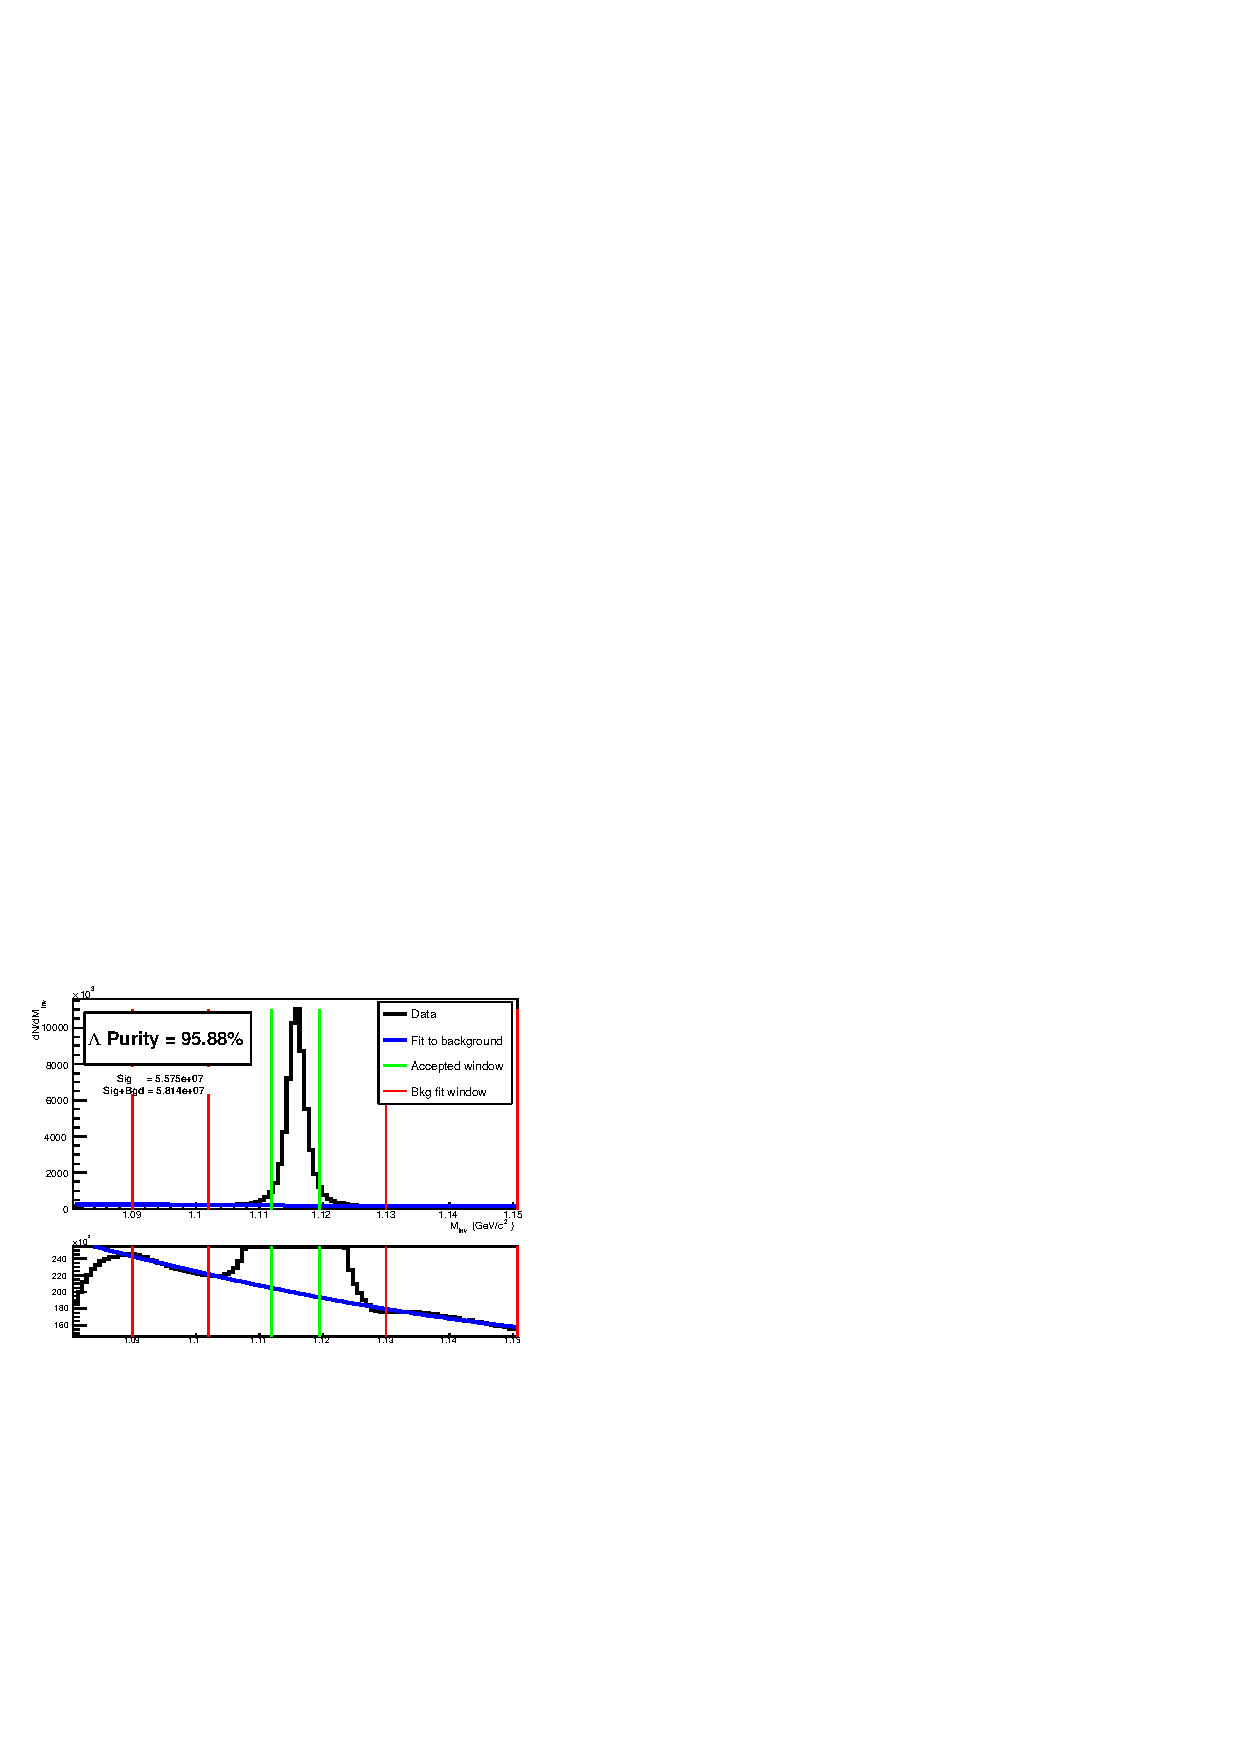
\includegraphics[width=0.49\linewidth]{/home/jesse/Analysis/FemtoAnalysis/LamKPublication/Figures/PDF/LamPurity_LamK0.pdf}}
   %%----start of second subfigure---  
-  \subfigure[$\pi^{+}\pi^{-}$ invariant mass distribution where the \Ks peak is seen.]{
+  \subfigure{
     \label{fig:Purity:b}
     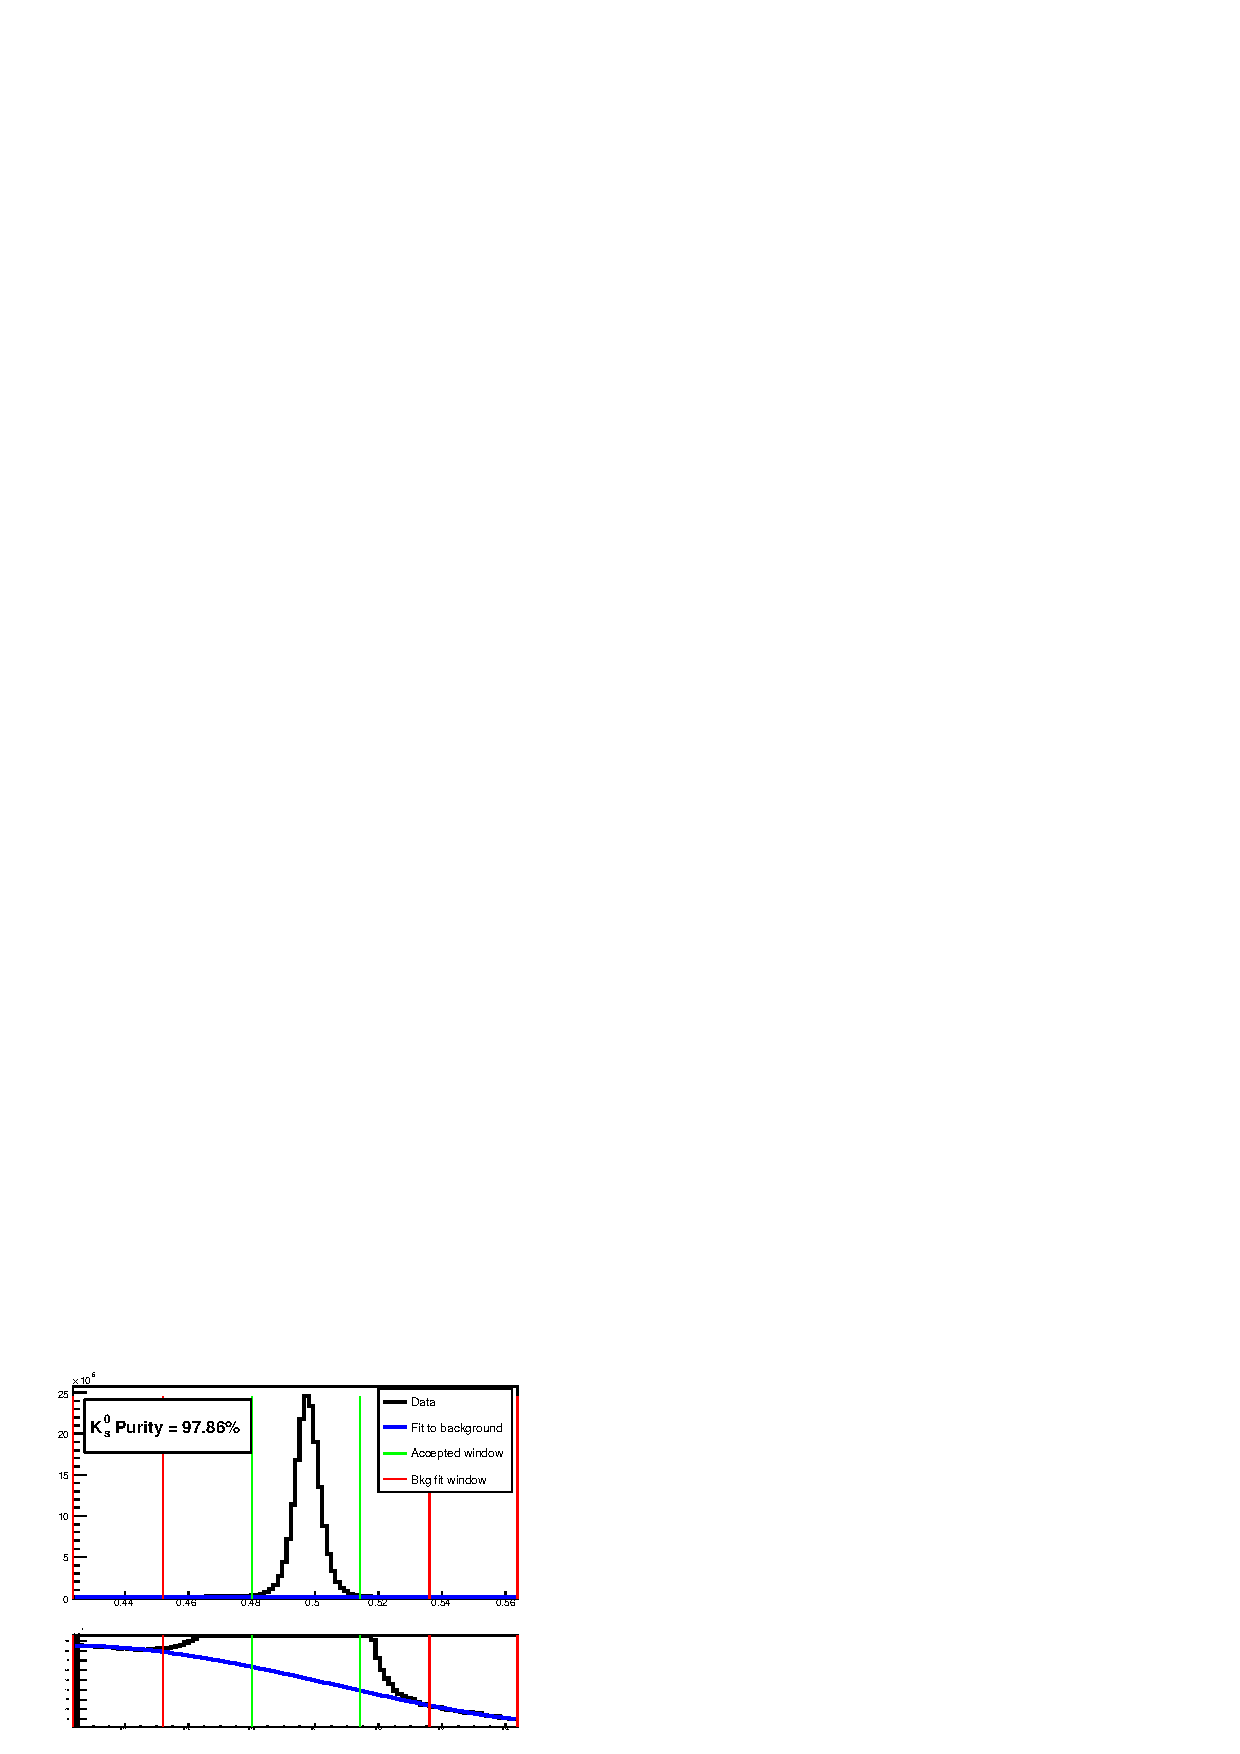
\includegraphics[width=0.49\linewidth]{/home/jesse/Analysis/FemtoAnalysis/LamKPublication/Figures/PDF/K0Purity_LamK0.pdf}}
   %%----overall caption----
@@ -506,7 +506,7 @@
 %************************************************************************************************************************
 \subsection{Correlation function}
 \label{sec:CorrelationFunction}
-The two-particle correlation function, $C_{ab}(\vec{\mathrm{p}}_{a},\vec{\mathrm{p}}_{b})$, is defined as the ratio of the probability of simultaneously measuring two particles with momenta $p_{a}$ and $p_{b}$, to the product of the single-particle probabilities.
+The two-particle correlation function for particles $a$ and $b$, $C_{ab}(\vec{\mathrm{p}}_{a},\vec{\mathrm{p}}_{b})$, is defined as the ratio of the probability of simultaneously measuring two particles with momenta $p_{a}$ and $p_{b}$, to the product of the single-particle probabilities.
 These probabilities are directly related to the covariant two-particle spectrum, $E_{a}E_{b}\frac{dN_{ab}}{d^{3}p_{a}d^{3}p_{b}}$, and the single-particle spectra, $E_{a(b)}\frac{dN_{a(b)}}{d^{3}p_{a(b)}}$, and the correlation function may be written
 \begin{equation}
   C_{ab}(\vec{\mathrm{p}}_{a},\vec{\mathrm{p}}_{b}) = \frac{E_{a}E_{b}\frac{dN_{ab}}{d^{3}p_{a}d^{3}p_{b}}}{\big( E_{a}\frac{dN_{a}}{d^{3}p_{a}} \big) \big( E_{b}\frac{dN_{b}}{d^{3}p_{b}} \big)},
@@ -609,7 +609,7 @@
 \label{eqn:ResidualsTransform}
 \end{equation}
 where $T(k^{*}_{ij},k^{*}_{\Lambda\mathrm{K}})$ is the transform matrix, which is generated with the THERMINATOR 2~\cite{Chojnacki:2011hb} simulation. 
-The transform matrix describes the decay kinematics of the parent system into the daughter, and is essentially an unnormalized probability distribution mapping the \kstar of the parent pair to that of the daughter pair when one or both parents decay (see Ref.~\cite{Kisiel:2014mma} for more details).
+The transform matrix describes the decay kinematics of the parent system into the daughter, and is essentially an unnormalized probability distribution mapping the \kstar of the parent pair to that of the daughter pair when one or both parents decay (see~\cite{Kisiel:2014mma} for more details).
 
 The contribution of a parent system (e.g., $\Sigma^{0}$\KchP) to the daughter correlation function (e.g., \LamKchP) is determined by modeling the parent system's correlation function and running it through the appropriate transform matrix.
 Since the interactions between these particles are not known, some assumptions must be made.
@@ -656,15 +656,16 @@
 More simply, this amounts to $\lambda_{\mathrm{Fakes}} = 1.0-PP_{\Lambda\mathrm{K}}$.
 The correlations in both of these categories (``Other'' and ``Fakes'') are assumed to average to unity, and pairs in these categories therefore only contribute by attenuating the signal. 
 
-
-\begin{table}[htbp]
+%%%%%%%%%%%%%%%%%%%%%%%%%%%%%%%%%%%%%%%%%%%%%%%%%%%%%%%%%%%%%%%%%%%%%%%%%%%%%%%%%%%%%%%%%%%%%%%%%%%%%%%%%%%%%%%%%%%%%%%%%%%%%%%%%%%%%
+\begin{comment}
+\begin{table}[htbp] 
  \centering
  \caption{Weight parameters ($\lambda_{ij}$) for the individual components of the \LamK correlation functions}
  \renewcommand{\arraystretch}{1.2}
 
- \begin{tabular}{|c|cV{4.0}c|cV{4.0}c|cV{4.0}c|c|}
+ \begin{tabular}{c|cV{4.0}c|cV{4.0}c|cV{4.0}c|c}
   \multicolumn{2}{c}{\LamKchP} & \multicolumn{2}{c}{\ALamKchM} & \multicolumn{2}{c}{\LamKchM} & \multicolumn{2}{c}{\ALamKchP} \\
-  \hline
+  \hlineB{3.0}
   \textbf{Source} & \textbf{$\lambda$ value} & \textbf{Source} & \textbf{$\lambda$ value} & \textbf{Source} & \textbf{$\lambda$ value} & \textbf{Source} & \textbf{$\lambda$ value} \\
   \hlineB{3.0}
   Primary & 0.527 & Primary & 0.526 & Primary & 0.526 & Primary & 0.527 \\
@@ -678,20 +679,60 @@
   \multicolumn{8}{c}{} \\
 
   \multicolumn{2}{c}{} & \multicolumn{2}{c}{\LamKs} & \multicolumn{2}{c}{\ALamKs} & \multicolumn{2}{c}{} \\ 
-  \cline{3-6}
-  \multicolumn{2}{c|}{} & \textbf{Pair System} & \textbf{$\lambda$ value} & \textbf{Pair System} & \multicolumn{1}{c|}{\textbf{$\lambda$ value}} & \multicolumn{2}{c}{} \\
   \clineB{3-6}{3.0}
-  \multicolumn{2}{c|}{} & Primary & 0.543 & Primary & \multicolumn{1}{c|}{0.544} & \multicolumn{2}{c}{} \\  
-  \multicolumn{2}{c|}{} & $\Sigma^{0}$K$^{0}_{\mathrm{S}}$ & 0.120 & $\overline{\Sigma}^{0}$K$^{0}_{\mathrm{S}}$ & \multicolumn{1}{c|}{0.120} & \multicolumn{2}{c}{} \\  
-  \multicolumn{2}{c|}{} & $\Xi^{0}$K$^{0}_{\mathrm{S}}$ & 0.042 & $\overline{\Xi}^{0}$K$^{0}_{\mathrm{S}}$ & \multicolumn{1}{c|}{0.039} & \multicolumn{2}{c}{} \\  
-  \multicolumn{2}{c|}{} & $\Xi^{-}$K$^{0}_{\mathrm{S}}$ & 0.054 & $\overline{\Xi}^{+}$K$^{0}_{\mathrm{S}}$ & \multicolumn{1}{c|}{0.050} & \multicolumn{2}{c}{} \\  
-  \multicolumn{2}{c|}{} & Other & 0.194 & Other & \multicolumn{1}{c|}{0.199} & \multicolumn{2}{c}{} \\  
-  \multicolumn{2}{c|}{} & Fakes & 0.048 & Fakes & \multicolumn{1}{c|}{0.048} & \multicolumn{2}{c}{} \\
+  %\multicolumn{2}{c|}{} & \textbf{Source} & \textbf{$\lambda$ value} & \textbf{Source} & \multicolumn{1}{c|}{\textbf{$\lambda$ value}} & \multicolumn{2}{c}{} \\
+  \multicolumn{2}{c}{} & \textbf{Source} & \textbf{$\lambda$ value} & \textbf{Source} & \multicolumn{1}{c}{\textbf{$\lambda$ value}} & \multicolumn{2}{c}{} \\
+  \clineB{3-6}{3.0}
+  \multicolumn{2}{c}{} & Primary & 0.543 & Primary & \multicolumn{1}{c}{0.544} & \multicolumn{2}{c}{} \\  
+  \multicolumn{2}{c}{} & $\Sigma^{0}$K$^{0}_{\mathrm{S}}$ & 0.120 & $\overline{\Sigma}^{0}$K$^{0}_{\mathrm{S}}$ & \multicolumn{1}{c}{0.120} & \multicolumn{2}{c}{} \\  
+  \multicolumn{2}{c}{} & $\Xi^{0}$K$^{0}_{\mathrm{S}}$ & 0.042 & $\overline{\Xi}^{0}$K$^{0}_{\mathrm{S}}$ & \multicolumn{1}{c}{0.039} & \multicolumn{2}{c}{} \\  
+  \multicolumn{2}{c}{} & $\Xi^{-}$K$^{0}_{\mathrm{S}}$ & 0.054 & $\overline{\Xi}^{+}$K$^{0}_{\mathrm{S}}$ & \multicolumn{1}{c}{0.050} & \multicolumn{2}{c}{} \\  
+  \multicolumn{2}{c}{} & Other & 0.194 & Other & \multicolumn{1}{c}{0.199} & \multicolumn{2}{c}{} \\  
+  \multicolumn{2}{c}{} & Fakes & 0.048 & Fakes & \multicolumn{1}{c}{0.048} & \multicolumn{2}{c}{} \\
   \clineB{3-6}{3.0} 
  \end{tabular}
  %\caption{$\lambda$ values for the individual components of the \LamK correlation functions.}
  \label{tab:LambdaValues_3Res}
 \end{table}
+\end{comment}
+%%%%%%%%%%%%%%%%%%%%%%%%%%%%%%%%%%%%%%%%%%%%%%%%%%%%%%%%%%%%%%%%%%%%%%%%%%%%%%%%%%%%%%%%%%%%%%%%%%%%%%%%%%%%%%%%%%%%%%%%%%%%%%%%%%%%%
+
+\begin{table}[htbp] 
+ \centering
+ \caption{Weight parameters ($\lambda_{ij}$) for the individual components of the \LamK correlation functions}
+ \renewcommand{\arraystretch}{1.2}
+
+ \begin{tabular}{c|c c c|c c c|c c c|c}
+  \multicolumn{2}{c}{\LamKchP} & \multicolumn{1}{c}{} & \multicolumn{2}{c}{\ALamKchM} & \multicolumn{1}{c}{} & \multicolumn{2}{c}{\LamKchM} & \multicolumn{1}{c}{} & \multicolumn{2}{c}{\ALamKchP} \\
+  \clineB{1-2}{3.0} \clineB{4-5}{3.0} \clineB{7-8}{3.0} \clineB{10-11}{3.0}
+  Source & $\lambda$ value & \multicolumn{1}{c}{} & Source & $\lambda$ value & \multicolumn{1}{c}{} & Source & $\lambda$ value & \multicolumn{1}{c}{} & Source & $\lambda$ value \\
+  \clineB{1-2}{3.0} \clineB{4-5}{3.0} \clineB{7-8}{3.0} \clineB{10-11}{3.0}
+  Primary & 0.527 & \multicolumn{1}{c}{} & Primary & 0.526 & \multicolumn{1}{c}{} & Primary & 0.526 & \multicolumn{1}{c}{} & Primary & 0.527 \\
+  $\Sigma^{0}$K$^{+}$ & 0.111 & \multicolumn{1}{c}{} & $\overline{\Sigma}^{0}$K$^{-}$ & 0.110 & \multicolumn{1}{c}{} & $\Sigma^{0}$K$^{-}$ & 0.110 & \multicolumn{1}{c}{} & $\overline{\Sigma}^{0}$K$^{+}$ & 0.111 \\  
+  $\Xi^{0}$K$^{+}$ & 0.039 & \multicolumn{1}{c}{} & $\overline{\Xi}^{0}$K$^{-}$ & 0.035 & \multicolumn{1}{c}{} & $\Xi^{0}$K$^{-}$ & 0.038 & \multicolumn{1}{c}{} & $\overline{\Xi}^{0}$K$^{+}$ & 0.036 \\  
+  $\Xi^{-}$K$^{+}$ & 0.050 & \multicolumn{1}{c}{} & $\overline{\Xi}^{+}$K$^{-}$ & 0.046 & \multicolumn{1}{c}{} & $\Xi^{-}$K$^{-}$ & 0.050 & \multicolumn{1}{c}{} & $\overline{\Xi}^{+}$K$^{+}$ & 0.046 \\  
+  Other & 0.226 & \multicolumn{1}{c}{} & Other & 0.235 & \multicolumn{1}{c}{} & Other & 0.228 & \multicolumn{1}{c}{} & Other & 0.233 \\  
+  Fakes & 0.048 & \multicolumn{1}{c}{} & Fakes & 0.048 & \multicolumn{1}{c}{} & Fakes & 0.048 & \multicolumn{1}{c}{} & Fakes & 0.048 \\
+  \cline{1-2} \cline{4-5} \cline{7-8} \cline{10-11}
+  
+  \multicolumn{11}{c}{} \\
+
+  \multicolumn{3}{c}{} & \multicolumn{2}{c}{\LamKs} & \multicolumn{1}{c}{} & \multicolumn{2}{c}{\ALamKs} & \multicolumn{3}{c}{} \\ 
+  \clineB{4-5}{3.0} \clineB{7-8}{3.0}
+  \multicolumn{3}{c}{} & Source & $\lambda$ value & \multicolumn{1}{c}{} & Source & \multicolumn{1}{c}{$\lambda$ value} & \multicolumn{3}{c}{} \\
+  \clineB{4-5}{3.0} \clineB{7-8}{3.0}
+  \multicolumn{3}{c}{} & Primary & 0.543 & \multicolumn{1}{c}{} & Primary & \multicolumn{1}{c}{0.544} & \multicolumn{3}{c}{} \\  
+  \multicolumn{3}{c}{} & $\Sigma^{0}$K$^{0}_{\mathrm{S}}$ & 0.120 & \multicolumn{1}{c}{} & $\overline{\Sigma}^{0}$K$^{0}_{\mathrm{S}}$ & \multicolumn{1}{c}{0.120} & \multicolumn{3}{c}{} \\  
+  \multicolumn{3}{c}{} & $\Xi^{0}$K$^{0}_{\mathrm{S}}$ & 0.042 & \multicolumn{1}{c}{} & $\overline{\Xi}^{0}$K$^{0}_{\mathrm{S}}$ & \multicolumn{1}{c}{0.039} & \multicolumn{3}{c}{} \\  
+  \multicolumn{3}{c}{} & $\Xi^{-}$K$^{0}_{\mathrm{S}}$ & 0.054 & \multicolumn{1}{c}{} & $\overline{\Xi}^{+}$K$^{0}_{\mathrm{S}}$ & \multicolumn{1}{c}{0.050} & \multicolumn{3}{c}{} \\  
+  \multicolumn{3}{c}{} & Other & 0.194 & \multicolumn{1}{c}{} & Other & \multicolumn{1}{c}{0.199} & \multicolumn{3}{c}{} \\  
+  \multicolumn{3}{c}{} & Fakes & 0.048 & \multicolumn{1}{c}{} & Fakes & \multicolumn{1}{c}{0.048} & \multicolumn{3}{c}{} \\
+  \cline{4-5} \cline{7-8}
+ \end{tabular}
+ %\caption{$\lambda$ values for the individual components of the \LamK correlation functions.}
+ \label{tab:LambdaValues_3Res}
+\end{table}
+
 
 %************************************************************************************************************************
 \subsection{Momentum resolution corrections}
@@ -745,7 +786,7 @@
   \includegraphics[width=\textwidth]{/home/jesse/Analysis/FemtoAnalysis/AnalysisNotes/5_Fitting/5.5_NonFlatBackground/Figures/BgdwFitOnly_RandomEPs_NumWeight1_Full_AllAnwConj_1030_3050_CustomRebin.pdf}
   \caption[Backgrounds with THERMINATOR 2]
   {
-  (Color online) THERMINATOR 2 simulation (open triangles) together with experimental data (closed circles).  
+  (Color online) THERMINATOR 2 simulation (open squares) together with experimental data (closed circles).  
   Results are shown for \LamKchP (left), \LamKchM (middle), and \LamKs (right).
   A $6^{\mathrm{th}}$-order polynomial fit to the simulation is shown as a dashed curve.  
   This polynomial is scaled to match the experimental data.  
@@ -811,11 +852,11 @@
 
 \begin{table}[htbp]
  \centering 
- \caption[\LamK systematics]{Selection parameter variation for the study of systematic uncertainties in the analysis. In the table, the shorthand used is as follows: $PA$ = pointing angle; PV = primary vertex; DCA = distance of closest approach; $\overline{\Delta\mathbf{r}}$ = average separation}
+ \caption[\LamK systematics]{Selection parameter variation for the study of systematic uncertainties in the analysis. In the table, the shorthand used is as follows: PA~=~pointing angle; PV~=~primary vertex; DCA~=~distance of closest approach; $\overline{\Delta\mathbf{r}}$~=~average separation}
   \renewcommand{\arraystretch}{1.2}
   \begin{tabular}{l|r}
    \hlineB{3.0} 
-   \multicolumn{2}{c}{\textbf{\LamKs systematics}} \\
+   \multicolumn{2}{c}{\LamKs} \\
    \hlineB{3.0}  
    DCA to PV \LamALam & $<$ [0.4, 0.5, 0.6] cm \\
    \hline
@@ -825,9 +866,9 @@
    \hline
    DCA \Ks Daughters & $<$ [0.2, 0.3, 0.4] cm \\
    \hline
-   $\cos(\theta_{PA})$ \LamALam to PV & $>$ [0.9992, 0.9993, 0.9994] \\
-   \hline
-   $\cos(\theta_{PA})$ \Ks to PV & $>$ [0.9992, 0.9993, 0.9994] \\
+   $\cos(\theta_{\mathrm{PA}})$ \LamALam to PV & $>$ [0.9992, 0.9993, 0.9994] \\
+   \hline
+   $\cos(\theta_{\mathrm{PA}})$ \Ks to PV & $>$ [0.9992, 0.9993, 0.9994] \\
    \hline
    DCA to PV of $\mathrm{p}\,(\overline{\mathrm{p}})$ Daughter of \LamALam & $>$ [0.05, 0.1, 0.2] cm \\
    \hline
@@ -840,13 +881,13 @@
    $\overline{\Delta\mathbf{r}}$ of Like-Charge Daughters & $>$ [5, 6, 7] cm \\
    
    \hlineB{3.0} 
-   \multicolumn{2}{c}{\textbf{\LamKpm systematics}} \\
+   \multicolumn{2}{c}{\LamKpm} \\
    \hlineB{3.0}  
    DCA \LamALam to PV & $<$ [0.4, 0.5, 0.6] cm \\ 
    \hline
    DCA \LamALam Daughters & $<$ [0.3, 0.4, 0.5] cm \\
    \hline
-   $\cos(\theta_{PA})$ \LamALam to PV & $>$ [0.9992, 0.9993, 0.9994] \\
+   $\cos(\theta_{\mathrm{PA}})$ \LamALam to PV & $>$ [0.9992, 0.9993, 0.9994] \\
    \hline
    DCA to PV of $\mathrm{p}\,(\overline{\mathrm{p}})$ Daughter of \LamALam &  $>$ [0.05, 0.1, 0.2] cm \\
    \hline
@@ -904,8 +945,8 @@
   \caption[Extracted Scattering Parameters]
   {
   (Color online) Extracted fit parameters for all of the \LamK systems.  
-  [Left]: $\Im f_{0}$ and $\Re f_{0}$, together with $d_{0}$ to the right for the \LamKchP (circles), \LamKchM (squares) and \LamKs (triangles) systems.  
-  [Right]: $\lambda$ and radius parameters for the 0--10\% (circles), 10--30\% (squares), and 30--50\% (triangles) centrality intervals.  
+  (Left) The scattering parameters, $\Im f_{0}$ and $\Re f_{0}$, together with $d_{0}$ to the right, for the \LamKchP (circles), \LamKchM (squares) and \LamKs (stars) systems.  
+  (Right) The $\lambda_{\mathrm{Fit}}$ and radius parameters for the 0--10\% (circles), 10--30\% (squares), and 30--50\% (stars) centrality intervals.  
   In the fit, all \LamK systems share common radii.
   The cross~\cite{Liu:2006xja} and X~\cite{Mai:2009ce} points show theoretical predictions made using chiral perturbation theory.
   }
@@ -921,7 +962,7 @@
 As is the usual convention in femtoscopy, a positive $\Re(f_{0})$ signifies that the effect of the interaction is attractive, while a negative $\Re(f_{0})$ signifies a repulsive interaction.
 Therefore, the femtoscopic signals from this analysis demonstrate that the strong interaction acts repulsively in the \LamKchP system, and acts attractively in the \LamKchM and \LamKs systems.
 
-In Figure~\ref{fig:ScattParams_3Res} (left), the predictions of Ref.~\cite{Liu:2006xja} do not distinguish the K\Lam and K\ALam interactions and results are shown for two different parameter sets, whereas Ref.~\cite{Mai:2009ce} offers unique K\Lam and $\overline{\mathrm{K}}$\Lam scattering parameters for a single parameter set. 
+In Fig.~\ref{fig:ScattParams_3Res} (left), the predictions of~\cite{Liu:2006xja} do not distinguish the K\Lam and K\ALam interactions and results are shown for two different parameter sets, whereas~\cite{Mai:2009ce} offers unique K\Lam and $\overline{\mathrm{K}}$\Lam scattering parameters for a single parameter set. 
 In all cases, the predicted scattering parameters have both positive real and imaginary components, which is clearly inconsistent with the \LamKchP system.
 Past studies of kaon-proton scattering found the K$^{-}$--p interaction to be attractive, and that of the K$^{+}$--p to be repulsive~\cite{Humphrey:1962zz, Hadjimichef:2002xe, Ikeda:2012au}.
 With respect to the kaons, this is similar to the current finding of an attractive \Lam--\KchM interaction and a repulsive \Lam--\KchP interaction.
@@ -950,7 +991,7 @@
 For non-identical particle pairs, to be more directly analogous to the single particle \mt, the definition of the pair transverse mass used in this study is
 \begin{equation}
 \begin{aligned}
- m_{\mathrm{T, pair}}^{2} &= \left( \frac{m_{\mathrm{inv}}}{2} \right)^{2} + \left( \frac{1}{2} |\textbf{\textit{p}}_{\mathrm{T,1}} + \textbf{\textit{p}}_{\mathrm{T,2}}| \right)^{2} = (K^{0})^{2} - (K^{3})^{2}, \quad \mathrm{where} ~~K^{\mu} \equiv \frac{1}{2} \left( p_{1}^{\mu} + p_{2}^{\mu} \right)
+ m_{\mathrm{T, pair}}^{2} &= \left( \frac{m_{\mathrm{inv}}}{2} \right)^{2} + \left( \frac{1}{2} |\textbf{\textit{p}}_{\mathrm{T,1}} + \textbf{\textit{p}}_{\mathrm{T,2}}| \right)^{2} = (K^{0})^{2} - (K^{3})^{2}, \quad \mathrm{where} ~~K^{\mu} \equiv \frac{1}{2} \left( p_{1}^{\mu} + p_{2}^{\mu} \right).
 \end{aligned}
 \label{eqn:PairmTv1}
 \end{equation}
@@ -968,7 +1009,7 @@
 
 A separation of the single-particle sources in the ``out" direction is expected for \LamK pairs at mid-rapidity in Pb--Pb collisions, as described above, and the experimental data support such an emission asymmetry.
 In addition to the ``size" of the emitting region (more precisely, the second moments of the emission functions) accessible with identical particle studies, non-identical particle correlations are sensitive to the relative emission shifts, i.e., the first moments of the emission function~\cite{Kisiel:2009eh}.
-The spherical harmonic decomposition of the correlation function offers an elegant method for extracting information about the emission asymmetries.
+The spherical harmonic decomposition of the correlation function offers an elegant method for extracting information about the emission asymmetries~\cite{Chajecki:2008vg, PhysRevC.72.054902, Kisiel:2009iw}.
 With this method, one can draw a wealth of information from just a few components of the decomposition.
 Particularly, the $l=0$, $m=0$ component, $C_{00}$, is similar to the one-dimensional correlation functions typically studied, and probes the overall size of the source.
 Of interest here, the real part of the $l=1$, $m=1$ component, $\Re C_{11}$, probes the asymmetry of the system in the ``out" direction; a non-zero value reveals the asymmetry. 
